%% proposal_1.tex
%% Core Proposal — CSP Project
%% 重构版：围绕"单次结构化的贝叶斯推断近似"这一核心问题展开
%% 中英混合写作

\documentclass[11pt,a4paper]{ctexart}

\usepackage{amsmath,amssymb}
\usepackage{array}
\usepackage{booktabs}
\usepackage{geometry}
\usepackage{graphicx}
\usepackage{hyperref}
\usepackage{xcolor}
\usepackage{tikz}
\usepackage{float}
\usepackage{enumitem}
\usepackage{caption}
\usepackage{subcaption}
\usetikzlibrary{arrows.meta,positioning,fit,calc}

\geometry{left=2.5cm,right=2.5cm,top=2.8cm,bottom=2.8cm}

\hypersetup{
    colorlinks=true,
    linkcolor=blue!60!black,
    citecolor=blue!60!black,
    urlcolor=blue!60!black
}

\tikzset{
    var/.style={circle,draw,thick,minimum size=8mm,inner sep=0pt},
    obs/.style={circle,draw,thick,fill=gray!25,minimum size=8mm,inner sep=0pt},
    tgt/.style={circle,draw,very thick,double,minimum size=8mm,inner sep=0pt},
    focus/.style={circle,draw=red!70!black,very thick,fill=red!10,minimum size=8mm,inner sep=0pt},
    shellzero/.style={draw=blue!70!black,very thick},
    shellone/.style={draw=teal!70!black,dashed,very thick},
    shelltwo/.style={draw=orange!70!black,dotted,very thick},
    fillin/.style={draw=orange!85!black,dashed,very thick},
    box/.style={draw,rounded corners,thick,fill=gray!8,inner sep=6pt,align=center},
    arr/.style={-{Latex[length=2.5mm]},thick},
    familybox/.style={draw,rounded corners,thick,inner sep=5pt,align=center,
        minimum width=2.8cm,minimum height=1.2cm}
}

\title{\textbf{Bounded Structural Inference over Factor Graphs}\\[4pt]
\large Core Proposal — CSP Project}
\author{}
\date{\today}

\begin{document}
\maketitle
\tableofcontents
\bigskip

% =============================================================
\section{科学问题}
\label{sec:question}
% =============================================================

\subsection{研究背景}

人类在复杂、结构化的环境中做出概率判断时，是否利用了环境的全局结构？这一问题是认知科学中 bounded rationality 研究的核心之一 \cite{Gigerenzer1995,Todd2007}。近年来，Wu et al.\ (2021) \cite{Wu2021} 在图结构上的函数学习任务中发现，人类的泛化行为可以用 Gaussian process 在图上的扩散来描述，且扩散范围系统性地低于全局最优——他们称之为"undergeneralization"。这表明，人类对结构信息的利用是\textbf{有界的、连续的、可量化的}，而不是全有或全无的。

本 proposal 将这一逻辑从函数学习推广到\textbf{概率推断}。我们选择 factor graph 上的软约束推断（以地图填色为操作化）作为实验范式，因为它同时具备两个理想特征：(1)~图结构提供了可操纵的全局依赖关系；(2)~精确推断（变量消除, variable elimination）提供了可计算的 normative baseline。

\subsection{核心问题定义}

本项目的核心科学问题是：

\begin{quote}
\textbf{当人类在图结构化的概率推断任务中报告对某个未观测变量的概率分布时，他们使用的是怎样的结构近似？}
\end{quote}

具体而言，我们区分三类可能的近似方式：
\begin{enumerate}[label=(\alph*)]
    \item \textbf{参数近似}（parameter approximation）：在正确的图结构上推断，但远端约束的影响随距离衰减——即内部表征了正确的拓扑，但对远端信息做了有界利用；
    \item \textbf{结构近似}（structure approximation）：改写了内部图结构——例如将图坍缩为以目标节点为中心的星形图，或将局部区域打包成一个紧凑的 cluster——然后在改写后的图上做精确或近精确推断；
    \item \textbf{纯局部推断}（local-only inference）：完全忽略远端结构，仅使用直接邻居信息。
\end{enumerate}

这三类近似对应于我们模型空间中的不同家族（§\ref{sec:models}），其预测在特定的图结构与证据条件下可以被行为上区分开。

\subsection{核心挑战}

从方法论角度，要回答上述问题面临四个主要挑战：

\begin{enumerate}
    \item \textbf{连续谱问题}：近似程度不是"有或无"而是一个连续谱，需要一个可识别的连续参数来量化。早期设计仅区分"精确推断"与"启发式搜索"，这是一个 binary contrast，无法捕捉连续的近似程度。
    \item \textbf{结构近似 vs.\ 参数近似的可分离性}：即便连续谱可量化，仍需区分"在正确图上做弱推断"（$M_\rho$）与"在错误图上做强推断"（$M_\mathrm{star}$, $M_\mathrm{cluster}$）。
    \item \textbf{参数混淆}：结构衰减参数 $\rho$ 和约束强度参数 $\beta_\mathrm{edge}$ 可能在行为预测上混淆，必须设计可以同时识别二者的刺激条件。
    \item \textbf{刺激设计}：需要系统性地筛选图/证据条件，使不同假设在目标节点后验上产生最大的可分离预测。
\end{enumerate}

\subsection{为什么重要}

本项目的意义在于提供一种\textbf{可操作、可量化的框架}来研究 bounded Bayesian inference 的内部结构。现有的 bounded rationality 研究大多聚焦于决策（choice under uncertainty）或函数学习（function learning），对\textbf{概率推断本身的结构近似}关注较少。通过引入 factor graph 上的精确 VE 模型族，我们可以：
\begin{itemize}
    \item 精确地量化被试的推断偏离精确后验的方式和程度；
    \item 区分不同近似策略（参数近似 vs.\ 结构改写 vs.\ 纯局部）；
    \item 连接 Wu et al.\ (2021) 的 undergeneralization 发现，将其扩展到更丰富的推断任务。
\end{itemize}

\subsection{与现有方法相比的新意}

与 Wu et al.\ \cite{Wu2021} 相比，本项目的新意在于：
\begin{itemize}
    \item Wu et al.\ 使用 GP diffusion 参数 $\alpha$ 描述在图上的 function generalization，而我们使用能量衰减参数 $\rho$ 描述 factor graph 上的 probabilistic inference；
    \item Wu et al.\ 的模型空间是单一家族（GP with varying $\alpha$），而我们的模型空间包含\textbf{质性不同的结构近似家族}（参数近似 vs.\ 结构改写），因此可以回答"人类用的是哪一类近似"这一更深层问题；
    \item 我们引入了系统化的刺激设计框架（rooted-shell descriptors, KL-based diagnostics），使实验设计可以被优化以最大化假设区分力。
\end{itemize}

\subsection{目标边界}

本 proposal 聚焦于以下范围，不展开次要问题：
\begin{itemize}
    \item 任务领域限于\textbf{反协调}（repulsive）图约束（地图填色）；是否推广到吸引（attractive）耦合是未来方向（§\ref{sec:discussion}）。
    \item 仅考虑\textbf{单次推断}（single-shot inference），不涉及序贯学习或 belief updating across trials。
    \item 不涉及 query heuristic 的独立研究（即自由选择查询顺序的策略）；这一问题作为未来方向在 §\ref{sec:discussion} 中讨论。
\end{itemize}


% =============================================================
\section{模型空间}
\label{sec:models}
% =============================================================

\subsection{统一框架：软约束因子图}

所有模型共享同一个基础表示。给定无向图 $G=(V,E)$，$|V|\in\{5,6,7,8\}$，每个节点 $X_i$ 取值于 $\{R,G,B\}$（三色），证据节点集 $E_\mathrm{obs}\subseteq V$ 带有 soft unary factor，未观测节点的联合分布为
\begin{equation}
\label{eq:joint}
p(\mathbf{x}\mid G,\boldsymbol{\lambda})
\;\propto\;
\prod_{e\in E_\mathrm{obs}} \phi_e(x_e)
\;\prod_{(u,v)\in E} \psi_{uv}(x_u,x_v),
\end{equation}
其中证据因子 $\phi_e(x_e)=\lambda_e(x_e)$ 编码观测节点的颜色偏好，边因子为
\begin{equation}
\label{eq:pairwise}
\psi_{uv}(x_u,x_v)
\;=\;
\exp\!\bigl[-\beta_\mathrm{edge}\,\mathbf{1}(x_u=x_v)\bigr],
\end{equation}
即同色受到强度为 $\beta_\mathrm{edge}$ 的软惩罚。默认 $\beta_\mathrm{edge}=4$。

\textbf{目标量}：给定证据后，目标节点 $X_i$ 的边缘后验 $P(X_i\mid E_\mathrm{obs})$。不同模型在如何计算（或近似）此量上有本质区别。

\subsection{六个候选模型家族}

基于 Analysis 4-1 的 agent taxonomy，我们保留以下 6 个模型家族。它们分为三大类：

\begin{center}
\begin{tikzpicture}[node distance=8mm and 12mm]
    \node[familybox,fill=blue!8] (exact) {$M_\mathrm{exact}$\\精确推断};
    \node[familybox,fill=green!8,below left=14mm and 5mm of exact] (rho) {$M_\rho$\\参数近似};
    \node[familybox,fill=green!8,below=6mm of rho] (rhobeta) {$M_{\rho,\beta}$\\参数+强度};
    \node[familybox,fill=green!8,above left=14mm and 5mm of exact] (m0) {$M_0$\\纯局部};
    \node[familybox,fill=orange!8,below right=14mm and 5mm of exact] (star) {$M_\mathrm{star}$\\星形改写};
    \node[familybox,fill=orange!8,below=6mm of star] (cluster) {$M_\mathrm{cluster}$\\局部 cluster};

    \draw[arr] (m0) -- node[above,sloped,font=\scriptsize]{$\rho\to 0$} (exact);
    \draw[arr] (rho) -- node[above,sloped,font=\scriptsize]{$\rho\to 1$} (exact);
    \draw[arr] (rhobeta) -- (rho);
    \draw[arr,dashed] (star) -- node[above,sloped,font=\scriptsize]{结构改写} (exact);
    \draw[arr,dashed] (cluster) -- node[above,sloped,font=\scriptsize]{结构改写} (exact);
\end{tikzpicture}
\end{center}

\subsubsection{$M_\mathrm{exact}$：精确推断（normative benchmark）}

在原始图 $G$ 上，通过变量消除（VE）或穷举求和计算精确边缘后验 $P(X_i\mid E_\mathrm{obs})$。这是所有比较的 normative baseline。

\begin{itemize}
    \item 内部图表征：保留完整 $G$
    \item 自由参数：$\beta_\mathrm{edge}$
    \item 对所有 rooted-shell descriptor 维度（D1, D2, D3）均敏感
\end{itemize}

\subsubsection{$M_0$：纯局部推断（local-only baseline）}

仅使用目标节点 $X_i$ 的直接观测邻居信息，等价于 $\rho=0$ 的特殊情形：
\begin{equation}
\label{eq:M0}
P_{M_0}(x_i\mid E_\mathrm{obs})
\;\propto\;
\prod_{j\in N(i)\cap E_\mathrm{obs}} \psi_{ij}(x_i,x_j).
\end{equation}
当目标节点没有直接观测邻居时，$M_0$ 输出均匀分布 $[1/3,1/3,1/3]$。

\begin{itemize}
    \item 内部图表征：保留 $G$，但仅激活 shell-0 边
    \item 自由参数：$\beta_\mathrm{edge}$
    \item 对 D1（target degree）敏感，对 D3（远端结构）不敏感
\end{itemize}

\paragraph{冗余排除.}
Analysis 4-4 证明：如果 proposed ``local log-evidence heuristic'' 对直接邻居的 log evidence 求和后做 exponentiate-and-normalise，其预测与 $M_0$ \textbf{数值上完全一致}（全刺激库上最大绝对差为 0.0）。因此不将其列为独立家族。

\subsubsection{$M_\rho$：有界变量消除（bounded VE, energy decay）}

核心连续参数模型。在原始图 $G$ 上做推断，但远端边的约束强度按距离衰减：
\begin{equation}
\label{eq:rho}
\psi^{(\rho,i)}_{uv}(x_u,x_v)
\;=\;
\exp\!\bigl[-\beta_\mathrm{edge}\,\rho^{s_i(u,v)}\,\mathbf{1}(x_u=x_v)\bigr],
\qquad
s_i(u,v)=\min\bigl(d(i,u),\,d(i,v)\bigr),
\end{equation}
其中 $d(\cdot,\cdot)$ 是图距离，$s_i(u,v)$ 是边 $(u,v)$ 到目标节点 $i$ 的 shell 距离。

\begin{table}[H]
\centering\small
\begin{tabular}{lll}
\toprule
$\rho$ 值 & 行为 & 等价模型 \\
\midrule
$\rho=0$ & 仅保留 shell-0 边，退化为纯局部推断 & $M_0$ \\
$0<\rho<1$ & 远端约束按距离指数衰减 & bounded VE \\
$\rho=1$ & 所有边保留完整约束 & $M_\mathrm{exact}$ \\
\bottomrule
\end{tabular}
\caption{$\rho$ 连续谱的两个极限与中间态。}
\end{table}

\begin{itemize}
    \item 内部图表征：保留完整 $G$，因子强度按 shell 距离衰减
    \item 自由参数：$\rho\in[0,1]$, $\beta_\mathrm{edge}$
    \item 类比于 Wu et al.\ 的 GP diffusion $\alpha$
\end{itemize}

\textbf{关键实现约束}：必须对\textbf{边能量} $\beta_\mathrm{edge}$ 做衰减，而不是对整个 factor 乘以距离相关常数。后者会被归一化抵消，导致不可识别（见 Design failures \#2）。

\subsubsection{$M_{\rho,\beta}$：有界 VE + 自由约束强度}

与 $M_\rho$ 使用相同的能量衰减公式 \eqref{eq:rho}，但显式允许 $\beta_\mathrm{edge}$ 作为自由参数变化（而非固定为 4）。

\begin{itemize}
    \item 动机：检验 $\rho$ 的结构衰减解释是否稳健——是否有可能通过调整全局约束强度 $\beta$ 来模拟结构衰减效应
    \item 自由参数：$\rho\in[0,1]$, $\beta_\mathrm{edge}$（联合估计）
    \item Analysis 4-3 显示：在 noiseless 条件下 $\rho$ 和 $\beta$ 可完全识别；在 noisy 条件下存在 tradeoff（MAE$(\hat\rho)=0.14$, MAE$(\hat\beta)=0.58$），但 star rewrite 家族在 $\beta$ 优化后仍与 attenuation 保持 JS $=0.027$ 的分离
\end{itemize}

\subsubsection{$M_\mathrm{star}$：目标中心星形改写（structure rewrite）}

图被内部坍缩为以目标节点为中心的星形图。每个非目标节点都直接连接到目标，有效约束强度按图距离衰减：
\begin{equation}
\label{eq:star}
\psi^{(\mathrm{star})}_{ij}(x_i,x_j)
\;=\;
\exp\!\biggl[-\frac{\beta_\mathrm{edge}}{d_G(i,j)}\,\mathbf{1}(x_i=x_j)\biggr],
\end{equation}
其中 $d_G(i,j)$ 是原始图 $G$ 上 $i$ 到 $j$ 的最短路径距离。

\begin{itemize}
    \item 内部图表征：\textbf{改写}为星形图，丢弃非目标节点间的所有连接
    \item 自由参数：$\beta_\mathrm{edge}$
    \item 心理学解释：所有远端影响被改写为直接的"目标中心推力"
    \item 对 D1 敏感（保留 degree 结构），对 D2（邻居间耦合）\textbf{不敏感}
\end{itemize}

\subsubsection{$M_\mathrm{cluster}$：局部 cluster / junction-lite 改写}

保留目标节点及其 shell-1 和 shell-2 邻居，并在 shell-1 内添加由共享 shell-2 邻居诱导的 fill-in 边，形成一个紧凑的局部 cluster 图。在该 cluster 图上做精确推断。

\begin{itemize}
    \item 内部图表征：\textbf{改写}为局部 cluster 图（保留到 shell-2 的结构，丢弃更远端的信息）
    \item 因子规则：原始局部边保留 $\beta_\mathrm{edge}$；fill-in 边也使用 $\beta_\mathrm{edge}$
    \item 自由参数：$\beta_\mathrm{edge}$
    \item 心理学解释：被试将局部 motif 打包为一个紧凑的 cluster 表征
    \item 对 D2（邻居间耦合）\textbf{非常敏感}
\end{itemize}

\subsection{模型家族总结}

\begin{table}[H]
\centering\small
\begin{tabular}{llll}
\toprule
家族 & 类型 & 图表征 & 自由参数 \\
\midrule
$M_\mathrm{exact}$ & normative benchmark & 完整 $G$ & $\beta_\mathrm{edge}$ \\
$M_0$ & 纯局部 baseline & $G$，仅 shell-0 边 & $\beta_\mathrm{edge}$ \\
$M_\rho$ & 固定图 + 参数衰减 & 完整 $G$，能量衰减 & $\rho,\,\beta_\mathrm{edge}$ \\
$M_{\rho,\beta}$ & 固定图 + 参数衰减 + 自由强度 & 完整 $G$，能量衰减 & $\rho,\,\beta_\mathrm{edge}$（联合估计） \\
$M_\mathrm{star}$ & 结构改写（星形） & 坍缩为 star & $\beta_\mathrm{edge}$ \\
$M_\mathrm{cluster}$ & 结构改写（cluster） & 局部 cluster + fill-in & $\beta_\mathrm{edge}$ \\
\bottomrule
\end{tabular}
\caption{六个候选模型家族总结。主模型为 $M_\rho$（连续参数近似），$M_0$ 和 $M_\mathrm{exact}$ 为两端 baseline，$M_\mathrm{star}$ 和 $M_\mathrm{cluster}$ 为结构改写竞争假设，$M_{\rho,\beta}$ 测试参数混淆。}
\label{tab:families}
\end{table}

\subsection{响应模型}

被试的概率报告 $y_t\in\Delta^2$（3 色概率向量）建模为：
\begin{equation}
\label{eq:response}
y_t \;\sim\; \mathrm{Dirichlet}\!\bigl(\kappa\cdot\tilde{b}_t(\Theta)\bigr),
\end{equation}
其中 $\tilde{b}_t$ 是模型预测的后验（在 response temperature $\beta_\mathrm{resp}$ 下 softened），$\kappa$ 是 Dirichlet 浓度参数。

\subsection{模型间逻辑关系}

六个家族不是完全独立的。Analysis 4 系列建立了以下关键关系：
\begin{enumerate}
    \item $M_\rho$ 在 $\rho=0$ 时退化为 $M_0$，在 $\rho=1$ 时退化为 $M_\mathrm{exact}$；
    \item $M_{\rho,\beta}$ 是 $M_\rho$ 的参数扩展，用于测试 $\rho$--$\beta$ 混淆；
    \item $M_\mathrm{star}$ 和 $M_\mathrm{cluster}$ 对图的\textbf{质性改写}不同于 $M_\rho$ 的量化衰减；
    \item 在当前刺激库上（600 个图/证据条件），$M_\mathrm{exact}$ 与 $M_\mathrm{star}$ 的平均 JS 散度为 0.114（最大），而 $M_\mathrm{exact}$ 与 $M_\rho$ 仅为 0.010（最小非零），说明\textbf{结构改写比参数衰减产生更强的行为预测差异}。
\end{enumerate}


% =============================================================
\section{典型案例与结构近似结果}
\label{sec:cases}
% =============================================================

本节用具体数值结果展示以上模型框架的可操作性。全部结果来自 Analysis 3（rooted-shell 刺激分类）和 Analysis 4 系列（家族 taxonomy、separability、identifiability）。

\subsection{Rooted-shell 刺激分类框架}

Analysis 3 建立了以目标节点 $X$ 为中心的 rooted-shell descriptor 框架，用三个维度刻画刺激结构：

\begin{itemize}
    \item \textbf{D1}：target degree $|S_1|$，即目标节点的直接邻居数；
    \item \textbf{D2}：shell-1 内部耦合 $e_{11}$，即 $S_1$ 内部的边数；
    \item \textbf{D3}：远端结构分类——
    \begin{itemize}
        \item D3-0: no remote structure ($|S_2|=0$)
        \item D3-1: tree-like remote ($|S_2|>0$, $e_{12}=|S_2|$, $e_{22}=0$)
        \item D3-2: strong remote（含多重回连或远端闭合）
    \end{itemize}
\end{itemize}

\paragraph{核心发现}：真正决定 $M_0$ vs $M_\mathrm{exact}$ 可分离性的不是 node count，而是 rooted descriptor。按 D3 分组的 $D_\mathrm{KL}(\tilde{b}_0\|\tilde{b}_1)$ 有清晰有序梯度：

\begin{table}[H]
\centering\small
\begin{tabular}{lccc}
\toprule
D3 class & rooted motifs 数 & 平均 $D_\mathrm{KL}$ & 最大 $D_\mathrm{KL}$ \\
\midrule
D3-0: no remote & 20 & 0.225 & 0.348 \\
D3-1: tree-like & 32 & 0.461 & 1.054 \\
D3-2: strong remote & 148 & 0.670 & 1.880 \\
\bottomrule
\end{tabular}
\caption{按 rooted remote-structure 分组的 $M_0$/$M_\mathrm{exact}$ 可分离性。}
\label{tab:d3_gradient}
\end{table}

\subsection{三个维度的 matched comparison}

Analysis 3 为 D1/D2/D3 各构造了至少一个 matched comparison（固定其余维度，只操纵一个）：

\begin{table}[H]
\centering\small
\begin{tabular}{llccl}
\toprule
维度 & matched pair & 操纵变量 & KL 变化 & 机制 \\
\midrule
D1 & RG018 $\to$ RG139 & $|S_1|$: $2\to 3$ & $0.237 \to 0.988$ & degree effect \\
D2 & RG088 $\to$ RG144 & $e_{11}$: $0\to 2$ & $1.093 \to 1.823$ & neighbour coupling \\
D3 & RG003 $\to$ RG058 & no-remote $\to$ strong & $0.132 \to 1.030$ & remote closure \\
\bottomrule
\end{tabular}
\caption{Matched comparison 结果。每一行固定其余 descriptor，只操纵目标维度。}
\end{table}

\subsection{六家族的 separability 概况}

Analysis 4-2 在 600 个图/证据条件上计算了 6 家族两两之间的 Jensen--Shannon 散度。关键结果：

\begin{table}[H]
\centering\small
\begin{tabular}{lc}
\toprule
家族对 & 平均 JS 散度 \\
\midrule
$M_\mathrm{exact}$ vs.\ $M_\mathrm{star}$ & 0.114 （最大——结构改写产生最强分离）\\
$M_\mathrm{star}$ vs.\ $M_\mathrm{cluster}$ & 0.104 \\
$M_\mathrm{exact}$ vs.\ $M_0$ & 0.049 \\
$M_\mathrm{star}$ vs.\ $M_{\rho,\beta}$ & 0.044 \\
$M_0$ vs.\ $M_\rho$ & 0.019 \\
$M_\mathrm{exact}$ vs.\ $M_\rho$ & 0.010 （最小——参数近似接近精确推断）\\
\bottomrule
\end{tabular}
\caption{六家族平均 JS 散度（完整 600 条件库）。结构改写家族产生的行为预测差异远大于参数衰减。}
\label{tab:js_matrix}
\end{table}

\subsection{$\rho$--$\beta$ 可识别性}

Analysis 4-3 对 $\rho$ 和 $\beta_\mathrm{edge}$ 的联合网格进行了参数恢复分析：
\begin{itemize}
    \item \textbf{Noiseless 恢复}：在 8 个高诊断力条件上，精确匹配率为 1.0（可识别）。
    \item \textbf{Noisy 恢复}：精确匹配率降至 0.3；MAE$(\hat\rho)=0.14$，MAE$(\hat\beta)=0.58$。
    \item \textbf{家族稳健性}：$\beta$ 优化后，attenuation 可完美坍缩到 $M_\mathrm{exact}$，但与 $M_\mathrm{star}$ 的最佳匹配仍留有 JS$=0.027$ 的间隙——结构改写家族比 $\rho$--$\beta$ 内部变化更稳健地可区分。
\end{itemize}


% =============================================================
\section{范式设计逻辑}
\label{sec:paradigm}
% =============================================================

本节解释\textbf{为什么}任务这样设计。核心原则是：

\begin{quote}
\textbf{范式设计的目标不是单纯拟合行为，而是最大化地区分不同科学假设。}
\end{quote}

\subsection{任务描述}

被试看到一个无向图（$|V|=6$--$8$），每个节点是一个国家，每条边表示相邻关系。一部分节点被预着色（证据）。被试需要报告一个指定目标节点颜色的完整概率分布（Red / Green / Blue），使用颜色轮。

\begin{center}
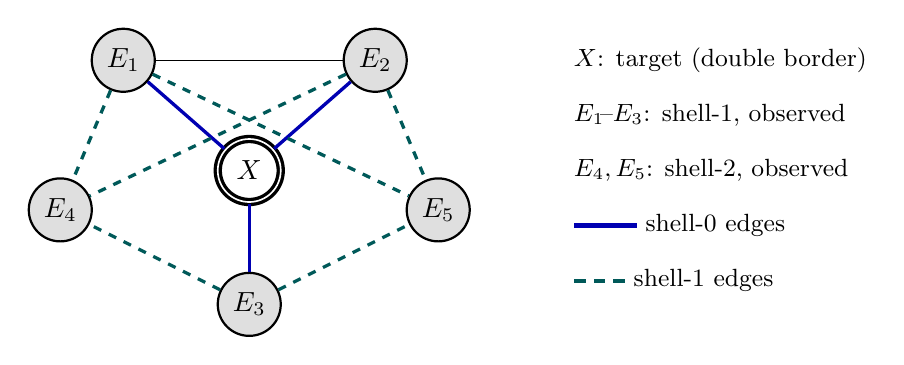
\begin{tikzpicture}[node distance=14mm and 14mm]
  % RG112: 6-node graph from analysis-3 selected stimuli (highest separability)
  % Target X at center; shell-1: E1, E2, E3; shell-2: E4, E5
  \node[tgt] (X) at (0,0) {$X$};
  \node[obs] (E1) at (-1.6,1.4)  {$E_1$};
  \node[obs] (E2) at (1.6,1.4)   {$E_2$};
  \node[obs] (E3) at (0,-1.7)    {$E_3$};
  \node[obs] (E4) at (-2.4,-0.5) {$E_4$};
  \node[obs] (E5) at (2.4,-0.5)  {$E_5$};
  % shell-0 edges (target to shell-1)
  \draw[shellzero] (X) -- (E1);
  \draw[shellzero] (X) -- (E2);
  \draw[shellzero] (X) -- (E3);
  % shell-1 internal edge
  \draw (E1) -- (E2);
  % shell-1 to shell-2 edges
  \draw[shellone] (E1) -- (E4);
  \draw[shellone] (E1) -- (E5);
  \draw[shellone] (E2) -- (E4);
  \draw[shellone] (E2) -- (E5);
  \draw[shellone] (E3) -- (E4);
  \draw[shellone] (E3) -- (E5);
  % annotations
  \node[align=left,anchor=west,font=\small] at (4.0,1.4)
    {$X$: target (double border)};
  \node[align=left,anchor=west,font=\small] at (4.0,0.7)
    {$E_1\!$--$E_3$: shell-1, observed};
  \node[align=left,anchor=west,font=\small] at (4.0,0.0)
    {$E_4, E_5$: shell-2, observed};
  \node[align=left,anchor=west,font=\small] at (4.0,-0.7)
    {\textcolor{blue!70!black}{\rule[0.4ex]{8mm}{1.5pt}} shell-0 edges};
  \node[align=left,anchor=west,font=\small] at (4.0,-1.4)
    {\textcolor{teal!70!black}{\rule[0.4ex]{1.5mm}{1.5pt}\hspace{1mm}\rule[0.4ex]{1.5mm}{1.5pt}\hspace{1mm}\rule[0.4ex]{1.5mm}{1.5pt}} shell-1 edges};
\end{tikzpicture}
\captionof{figure}{任务示意图。以 analysis-3 candidate stimulus RG112 为例：6 节点图，D1=3, D2=1, D3=strong-remote。被试需报告目标节点 $X$ 上 (R,G,B) 的完整概率分布。}
\end{center}

\subsection{为什么是 forced-target, one-pass, non-revisable}

设计失败 \#1 的教训：如果被试可以自由选择查询顺序并修改先前回答，VE 模型所依赖的 Markov 结构被破坏——elimination ordering 不再固定，fill-in 序列不再可解释，响应模型无法拟合。因此 Phase 1 必须满足：
\begin{itemize}
    \item \textbf{固定查询顺序}：fill-in $\mathrm{Fill}_t$ 和 clique size $\Omega_t$ 在每一步都是明确的；
    \item \textbf{一次通过、不可修改}：保持 Markov 结构和可拟合性。
\end{itemize}

\subsection{为什么是 soft constraint}

如果使用硬约束（hard constraint: $\mathbf{1}(x_u=x_v)=0$），$\rho$ 的连续谱退化——factor 取值非 0 即 1，无法通过 energy decay 生成连续的近似梯度。Soft constraint $\exp[-\beta_\mathrm{edge}\cdot\mathbf{1}(x_u=x_v)]$ 保证了 $\rho$ 的连续可识别性。

\subsection{为什么 conflicting evidence 优于 uniform evidence}

直觉上，如果所有证据节点都偏向同一种颜色（uniform evidence），远端约束在目标后验上的效应容易被局部证据信号淹没，导致不同 $\rho$ 水平的预测差异很小。Adaptive conflicting evidence 策略对每张 rooted graph 搜索一个非均匀的证据模板，使得
$\sum_{i<j} D_\mathrm{KL}(\tilde{b}_{\rho_i}\|\tilde{b}_{\rho_j})$
最大化，同时要求 $p_R$ 和 $H(\tilde{b}_\rho)$ 在 5 个 $\rho$ 水平上单调（容差 $5\times 10^{-4}$）。

Analysis 3 中的全部 200 个 rooted motifs 都使用该策略选出的最佳 evidence template 进行评估。结果表明，在 D3-2（strong remote）条件下，adaptive conflicting evidence 的平均 separability 达到 $D_\mathrm{KL}=0.670$（表~\ref{tab:d3_gradient}），远高于无远端结构（D3-0）条件下的 0.225——证实冲突证据确实能放大远端结构的诊断效应。

\subsection{试次选择与科学问题识别的关系}

不同类型的试次服务于不同的科学区分：

\begin{table}[H]
\centering\small
\begin{tabular}{ll}
\toprule
科学区分 & 关键试次类型 \\
\midrule
$H_0$ (local only) vs.\ $H_1$ (structure use) & equal-local 图对 \\
$\rho$ 连续谱的分辨 & high-evidence 强远端结构图 \\
参数近似 vs.\ 结构改写 & D2-diagnostic 条件（$M_\mathrm{star}$ 对 D2 不敏感） \\
$\rho$--$\beta$ 可识别 & 8 个高诊断力条件 panel \\
\bottomrule
\end{tabular}
\caption{试次类型与科学问题的对应关系。}
\end{table}


% =============================================================
\section{工程设计逻辑}
\label{sec:engineering}
% =============================================================

本节说明如何把上述科学目标落到可执行的实验设计上。

\subsection{刺激生成与筛选流程}

\begin{center}
\begin{tikzpicture}[node distance=10mm and 10mm]
    \node[box] (enum) {图枚举\\connected, 3-colorable\\$n=5,6,7,8$};
    \node[box,right=of enum] (root) {Rooted\\canonicalization\\以图中心为目标};
    \node[box,right=of root] (desc) {Rooted-shell\\descriptors\\D1/D2/D3 编码};
    \node[box,below=12mm of desc] (evid) {Adaptive conflicting\\evidence 优化\\$\max\sum_{i<j}D_\mathrm{KL}$};
    \node[box,left=of evid] (screen) {筛选\\$\Delta p_R^{\mathrm{high}}\ge 0.08$\\单调性检查};
    \node[box,left=of screen] (select) {Candidate\\stimulus set\\8 个图 $\times$ 3 个证据};

    \draw[arr] (enum) -- (root);
    \draw[arr] (root) -- (desc);
    \draw[arr] (desc) -- (evid);
    \draw[arr] (evid) -- (screen);
    \draw[arr] (screen) -- (select);
\end{tikzpicture}
\end{center}

\subsection{Informativeness 的度量依据}

两个层次的 informativeness：

\paragraph{$\rho$-层面（Analysis 3）.}
在 $M_0$--$M_\rho$--$M_\mathrm{exact}$ 谱上的总 pairwise KL 散度：
\[
\mathrm{Info}_\rho(G,\lambda)
\;=\;
\sum_{i<j} D_\mathrm{KL}\!\bigl(\tilde{b}_{\rho_i}(G,\lambda)\,\big\|\,\tilde{b}_{\rho_j}(G,\lambda)\bigr).
\]

\paragraph{Family-层面（Analysis 4）.}
在 6 家族之间的平均 JS 散度：
\[
\mathrm{Info}_\mathrm{fam}(G,\lambda)
\;=\;
\frac{1}{\binom{6}{2}}
\sum_{\substack{A,B\in\mathcal{M}\\A\neq B}}
\mathrm{JS}\!\bigl(\tilde{b}_A(G,\lambda),\,\tilde{b}_B(G,\lambda)\bigr).
\]

两个指标共同用于筛选最有诊断力的刺激条件。

\subsection{Synthetic model recovery}

刺激筛选完成后，在正式实验前需通过 synthetic recovery 验证模型可辨认性：
\begin{enumerate}
    \item 为每个生成模型模拟 60 个数据集：$y_t\sim\mathrm{Dirichlet}(\kappa\,b_t)$，$\kappa=80$；
    \item Leave-one-trial-out CV，最大化 $\sum_t\log p_\mathrm{Dir}(y_t;\kappa\tilde{b}_t(\Theta))$；
    \item BIC 选模型；
    \item 群体层面使用 protected exceedance probability (pxp)。
\end{enumerate}

\textbf{已验证结果}（Analysis 4-3）：在 8 个高诊断力条件的 diagnostic panel 上，noiseless 条件下 $\rho$--$\beta$ 联合参数的精确恢复率为 1.0；noisy 条件下精确匹配率降至 0.3，MAE$(\hat\rho)=0.14$，但家族层面（attenuation vs.\ star rewrite）的分离在 $\beta$ 优化后仍保持 JS$=0.027$。

\subsection{实验试次导出}

基于上述流程，最终导出的候选刺激集包含 8 个 rooted graph（覆盖 D1/D2/D3 三维、含 3 个 matched comparison），每图配 3 个证据水平。总试次数为 24（或按 balanced list 分为 6 份，每份 15 个试次）。

\begin{table}[H]
\centering\small
\begin{tabular}{lccccc}
\toprule
Graph & $n$ & D1 & D2 & D3 & high KL \\
\midrule
RG003 & 5 & 4 & 2 & no-remote & 0.132 \\
RG018 & 5 & 2 & 1 & tree-like & 0.237 \\
RG058 & 6 & 4 & 2 & strong & 1.030 \\
RG088 & 6 & 3 & 2 & strong & 1.823 \\
RG112 & 6 & 3 & 1 & strong & 1.880 \\
RG114 & 6 & 3 & 1 & strong & 1.771 \\
RG139 & 6 & 3 & 1 & tree-like & 0.988 \\
RG144 & 6 & 3 & 0 & strong & 1.093 \\
\bottomrule
\end{tabular}
\caption{候选刺激集。覆盖 D1=2--4, D2=0--2, 全部 3 个 D3 class。}
\end{table}

\subsection{理论目标到工程实现的映射}

\begin{table}[H]
\centering\small
\begin{tabular}{ll}
\toprule
理论目标 & 工程实现 \\
\midrule
区分 $H_0$ vs.\ $H_1$ & equal-local 图对 \\
量化 $\rho$ & high-evidence 强远端结构图 + energy decay 模型 \\
区分参数近似 vs.\ 结构改写 & D2-diagnostic 条件 \\
控制 $\rho$--$\beta$ 混淆 & 8 个高诊断力条件 + 联合参数恢复 \\
最大化 trial informativeness & adaptive conflicting evidence \\
验证可识别性 & synthetic model recovery (LOO-CV + BIC + pxp) \\
\bottomrule
\end{tabular}
\caption{从科学目标到工程实现的完整映射。}
\end{table}


% =============================================================
\section{讨论}
\label{sec:discussion}
% =============================================================

\subsection{当前方案的局限性}

\paragraph{近似形式可能过强.}
$M_\rho$ 假设 energy decay 是 $\rho^{s_i(u,v)}$ 的指数形式。人类的实际衰减函数可能是其他形式（如线性、阈值型）。当前框架下，这些替代形式被映射到 $M_\rho$ 的最佳拟合 $\hat\rho$ 上，可能引入系统性偏差。

\paragraph{模型假设可能过理想化.}
所有 6 个家族都假设被试在单个 trial 内使用\textbf{同一个}模型。实际上，被试可能在不同条件下切换策略，或使用多家族的混合。当前框架暂不处理 mixture 模型。

\paragraph{典型案例可能不足以覆盖真实复杂性.}
当前实验仅使用\textbf{反协调}（repulsive）map-colouring 任务。Analysis 4-7 指出，是否推广到\textbf{吸引}（attractive）耦合是检验家族 taxonomy 任务通用性的关键。

\paragraph{计算与实验条件限制.}
精确穷举仅在 $n\le 8$ 时可行（$3^8=6561$ 个赋值）。更大的图需要近似推断来计算模型预测，但目前所有预分析都使用 brute-force。

\paragraph{$\rho$--$\beta$ 混淆.}
Noisy recovery 显示 $\beta$ 的 MAE 为 0.58，显著高于 $\rho$ 的 0.14。在实验数据中，$\rho$ 与 $\beta$ 的联合估计需要限制在高诊断力条件 panel 上。

\subsection{未来工作方向}

\paragraph{更广泛的模型扩展.}
$M_\mathrm{star}$ 和 $M_\mathrm{cluster}$ 是结构改写家族的两个起点。更丰富的改写（如 junction tree 的局部近似、层次化 cluster）值得进一步探索。

\paragraph{更强的近似方法.}
Loopy BP 是一个自然的扩展——它在树图上等价于精确推断，在含环图上给出不同于 VE 的近似，可以作为 $M_\rho$ 之外的一种独立近似基线。

\paragraph{更真实的任务环境.}
Analysis 4-7 推荐 attractive graph labelling 作为下一个实验领域：它翻转了局部耦合语义（从排斥到吸引），同时保持了图推断的基本接口。

\paragraph{更自动化的 adaptive design.}
当前的 adaptive conflicting evidence 是 offline 优化。未来可以考虑 online adaptive design：根据被试前几个 trial 的回答，实时选择后续最 informative 的图/证据条件。

\paragraph{Query heuristic 的独立研究.}
在 Phase 2（free-query）中，被试自由选择查询顺序。分析被试选择的 elimination ordering 可以测试 Min-Degree（局部、低成本）vs.\ Min-Fill（one-step look-ahead）的策略偏好。跨 phase 预测是：在 Phase 1 中 $\hat\rho$ 更高的被试，在 Phase 2 中更倾向于 Min-Fill 策略。这是一个有趣的 individual-difference 分析方向，但不是当前 proposal 的主线。

\paragraph{Selection-plus-belief 范式.}
Analysis 4-5 初步评估了"先选目标节点、再报告 belief"的两阶段任务。结果显示 combined design 的平均 pairwise 家族分离（JS$=0.055$）远高于 belief-only（JS$=0.003$），但 recovery 优势有限（recovery diagonal $\approx 0.45$ vs.\ 0.59）。这适合作为 forced-target 范式的\textbf{定向扩展}，而非完全替代。

\bigskip
\noindent
总结：本 proposal 围绕"人类在图结构概率推断中使用怎样的结构近似"这一核心问题，建立了一个包含 6 个候选家族的模型空间，开发了基于 rooted-shell descriptor 和 KL-based diagnostics 的系统化刺激设计框架，并通过 4 轮 pre-analysis 验证了模型可识别性和刺激可分离性。下一步是实验接口开发、被试训练、pilot 数据采集和正式的 pre-registration。

\bibliographystyle{apalike}
\bibliography{library}

\end{document}
